\begin{activity} \label{A:12.1.2}  
\ba
\item In Figure~\ref{fig:12.1.level-curves} there are three sets of axes showing level
  curves for functions $f$, $g$, and $h$, respectively. Sketch at least six vectors
  in the gradient vector field for each function. In making your
  sketches, you don't have to worry about getting vector magnitudes
  precise, but you should ensure that the relative magnitudes (and directions) are
  correct for each function independently.
  \begin{figure}[h]
    \centering
    \parbox[t]{0.3\linewidth}{\centering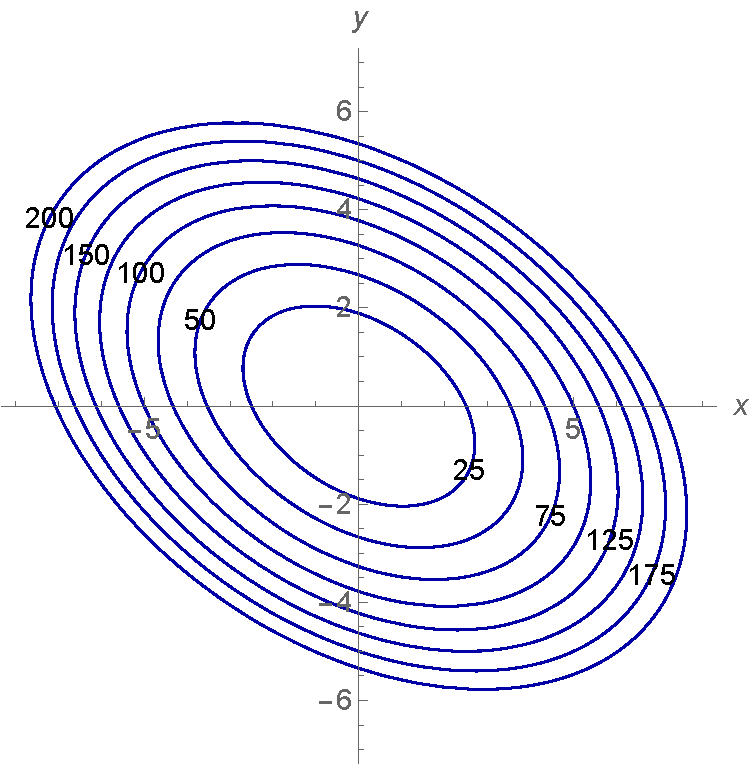
\includegraphics[width=\linewidth]{../figures/12_1_ellipses.pdf}\\\hspace{-4pt}$f$}\hspace{0.04\linewidth}\parbox[t]{0.3\linewidth}{\centering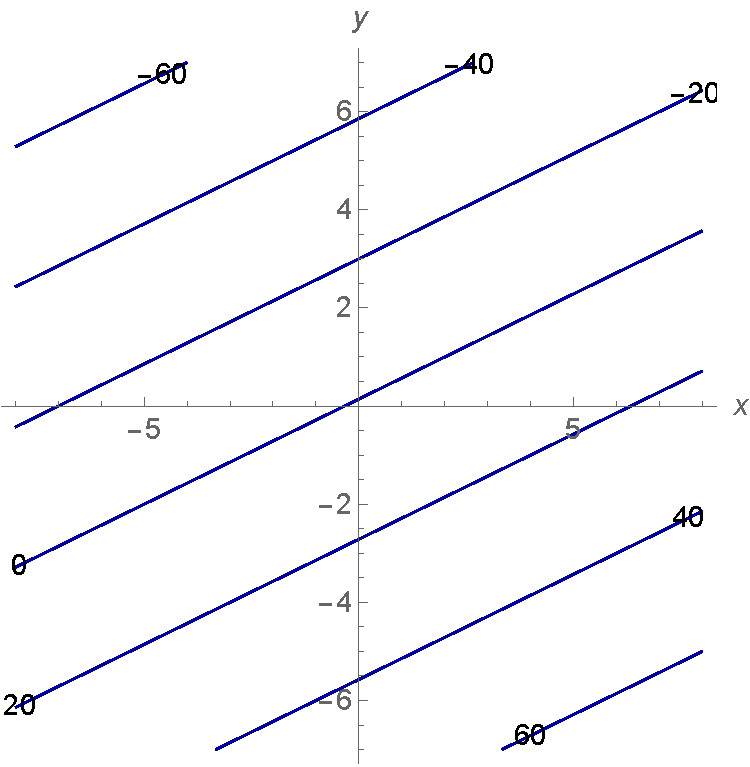
\includegraphics[width=\linewidth]{../figures/12_1_linear.pdf}\\\hspace{-4pt}$g$}\hspace{0.04\linewidth}\parbox[t]{0.3\linewidth}{\centering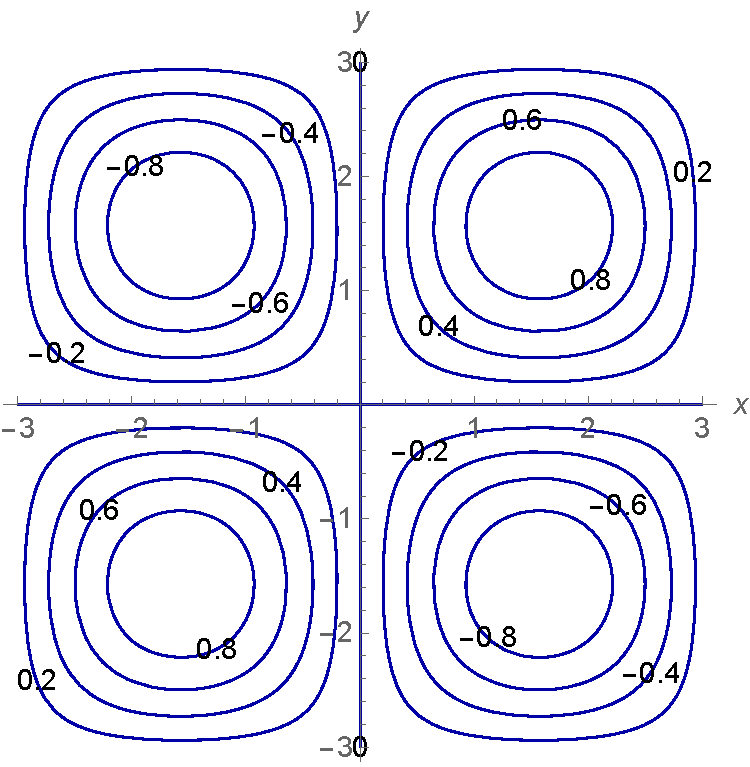
\includegraphics[width=\linewidth]{../figures/12_1_sine.pdf}\\\hspace{-3pt}$h$}
    \caption{Three sets of level curves}
    \label{fig:12.1.level-curves}
  \end{figure}
\item Verify that $\vF(x,y) = \langle 6xy,3x^2+9\sqrt{y}\rangle$ is a
  gradient vector field by finding a function $f$ such that $\nabla
  f(x,y) = \vF(x,y)$. For reasons originating in physics, such a
  function $f$ is called a \emph{potential function} for the vector
  field $\vF$.\label{part:A12.2-pot}
\item Is the function $f$ found in part \ref{part:A12.2-pot} unique?
  That is, can you find another function $g$ such that $\nabla g(x,y)
  = \vF(x,y)$ but $f\neq g$?
\item Is the vector field $\vF(x,y) = 6xy\vi +(2x+9\sqrt{y})\vj$ a
  gradient vector field? Why or why not?
\ea
\end{activity}
\begin{smallhint}

\end{smallhint}
\begin{bighint}

\end{bighint}
\begin{activitySolution}

\end{activitySolution}
\aftera
%%% Local Variables:
%%% mode: latex
%%% TeX-master: "../0_AC_MV"
%%% End:
